\chapter{Espacios vectoriales con producto interno}\label{evcpir}

Algunos espacios vectoriales poseen una propiedad particular llamada producto interno. La ventaja de esta propiedad es que nos permite medir longitudes y ángulos. Cuando un espacio vectorial posee producto interno, se facilitan considerablemente estas operaciones geométricas. En este capítulo definiremos el concepto de producto interno y estableceremos propiedades interesantes respecto a estos espacios vectoriales especiales.

\begin{definition}[Espacio vectorial con producto interno]
Sea $V$ un espacio vectorial real (Definición \ref{defespvectorial}). Un \textbf{producto interno} es una función $\langle \cdot, \cdot \rangle: V \times V \to \mathbb{R}$ que satisface:
\begin{enumerate}[$1.$]
    \item $\langle \mathbf{u},\mathbf{v} \rangle = \langle \mathbf{v},\mathbf{u} \rangle$ (Simetría)
    \item $\langle \mathbf{u} + \mathbf{v},\mathbf{w} \rangle = \langle \mathbf{u},\mathbf{w} \rangle + \langle \mathbf{v},\mathbf{w} \rangle$ (Linealidad en primera variable)
    \item $\langle k\mathbf{u},\mathbf{v} \rangle = k\langle \mathbf{u},\mathbf{v} \rangle$ para todo $k \in \mathbb{R}$ (Homogeneidad)
    \item $\langle \mathbf{u},\mathbf{u} \rangle \geq 0$ y $\langle \mathbf{u},\mathbf{u} \rangle = 0$ si y solo si $\mathbf{u} = \mathbf{0}$ (Positividad definida)
\end{enumerate}
\end{definition}

\begin{example}[Producto punto usual en $\mathbb{R}^2$]
Sean $\mathbf{u} = (u_1, u_2)$ y $\mathbf{v} = (v_1, v_2)$, el producto $$\langle \mathbf{u}, \mathbf{v} \rangle = u_1v_1 + u_2v_2$$ es un producto interno.
\begin{proof}
Verifiquemos los axiomas:
\begin{enumerate}[i.]
    \item $\langle \mathbf{u}, \mathbf{v} \rangle = u_1v_1 + u_2v_2 = v_1u_1 + v_2u_2 = \langle \mathbf{v}, \mathbf{u} \rangle$
    \item Para $\mathbf{w} = (w_1, w_2)$: \\
    $\langle \mathbf{u} + \mathbf{v}, \mathbf{w} \rangle = (u_1 + v_1)w_1 + (u_2 + v_2)w_2 = u_1w_1 + v_1w_1 + u_2w_2 + v_2w_2 = \langle \mathbf{u}, \mathbf{w} \rangle + \langle \mathbf{v}, \mathbf{w} \rangle$
    \item $\langle k\mathbf{u}, \mathbf{v} \rangle = (ku_1)v_1 + (ku_2)v_2 = k(u_1v_1 + u_2v_2) = k\langle \mathbf{u}, \mathbf{v} \rangle$
    \item $\langle \mathbf{u}, \mathbf{u} \rangle = u_1^2 + u_2^2 \geq 0$ y $u_1^2 + u_2^2 = 0$ si y solo si $u_1 = u_2 = 0$
\end{enumerate}
La generalización para $\mathbb{R}^n$ es $\langle \mathbf{u}, \mathbf{v} \rangle = \sum_{i=1}^n u_i v_i$ con $\mathbf{u} = (u_1, \dots, u_n)$, $\mathbf{v} = (v_1, \dots, v_n)$.
\end{proof}
\end{example}

\begin{example}[Producto interno no usual]
En $\mathbb{R}^2$, la función $\langle \mathbf{u}, \mathbf{v} \rangle = 2u_1v_1 + 3u_2v_2$ para $\mathbf{u} = (u_1, u_2)$, $\mathbf{v} = (v_1, v_2)$ define un producto interno. La verificación de axiomas es análoga al ejemplo anterior.
\end{example}

\begin{definition}[Norma inducida]
Dado $V$ con producto interno, la \textbf{norma inducida} de $\mathbf{u} \in V$ está dada por \(\|\mathbf{u}\| = \sqrt{\langle \mathbf{u}, \mathbf{u} \rangle}
.\)
\end{definition}

\begin{definition}[Bola unitaria]
La \textbf{bola unitaria} de $V$ es el conjunto \(
\mathcal{B}_V = \{ \mathbf{x} \in V : \|\mathbf{x}\| = 1 \}.\)
\begin{itemize}
    \item Con producto usual en $\mathbb{R}^2$: $\|\mathbf{u}\| = 1 \Rightarrow x^2 + y^2 = 1$ (circunferencia)
    \item Con producto $\langle \mathbf{u}, \mathbf{v} \rangle = 2u_1v_1 + 3u_2v_2$: $\|\mathbf{u}\| = 1 \Rightarrow 2x^2 + 3y^2 = 1$ (elipse)
\end{itemize}
\end{definition}

\begin{rem}[Ejemplos de productos internos]
\begin{enumerate}[1.]
    \item En $\mathcal{M}_n(\mathbb{R})$: $\langle A, B \rangle = \operatorname{Tr}(A^T B)$
    \item En $\mathbb{P}_n(\mathbb{R})$: $\langle p, q \rangle = \sum_{k=0}^n a_k b_k$ donde $p(x) = \sum_{k=0}^n a_k x^k$, $q(x) = \sum_{k=0}^n b_k x^k$
    \item En $\mathcal{C}[a,b]$: $\langle f, g \rangle = \int_a^b f(x)g(x)  dx$
\end{enumerate}
\end{rem}

\begin{definition}[Producto interno en espacios vectoriales complejos]
Sea $V$ un espacio vectorial complejo. Un \textit{producto interno} es una función $\langle \cdot, \cdot \rangle: V \times V \to \mathbb{C}$ que satisface:
\begin{enumerate}[$1.$]
    \item $\langle \mathbf{u}, \mathbf{v} \rangle = \overline{\langle \mathbf{v}, \mathbf{u} \rangle}$ (Simetría conjugada)
    \item $\langle \mathbf{u} + \mathbf{v}, \mathbf{w} \rangle = \langle \mathbf{u}, \mathbf{w} \rangle + \langle \mathbf{v}, \mathbf{w} \rangle$  (Aditividad)
    \item $\langle k\mathbf{u}, \mathbf{v} \rangle = k\langle \mathbf{u}, \mathbf{v} \rangle$ para todo $k \in \mathbb{C}$ (Homogeneidad en primera variable)
    \item $\langle \mathbf{u}, \mathbf{u} \rangle \geq 0$ y $\langle \mathbf{u}, \mathbf{u} \rangle = 0$ si y solo si $\mathbf{u} = \mathbf{0}$ (Positividad definida)
\end{enumerate}
\end{definition}

\begin{theorem}[Propiedades del producto interno en espacios vectoriales complejos]
Sea $V$ un espacio vectorial complejo con producto interno. Para todo $\mathbf{u}, \mathbf{v} \in V$ y $k \in \mathbb{C}$ se cumple que $\langle \mathbf{u}, k\mathbf{v} \rangle = \overline{k} \langle \mathbf{u}, \mathbf{v} \rangle$ (Conjugación en la segunda variable)
\end{theorem}

\begin{proof} Usando los axiomas del producto interno complejo:
    \begin{align*}
        \langle \mathbf{u}, k\mathbf{v} \rangle 
        &= \overline{\langle k\mathbf{v}, \mathbf{u} \rangle} && \text{(Simetría conjugada)} \\
        &= \overline{k \langle \mathbf{v}, \mathbf{u} \rangle} && \text{(Homogeneidad en 1ra variable)} \\
        &= \overline{k} \cdot \overline{\langle \mathbf{v}, \mathbf{u} \rangle} && \text{(Propiedad del conjugado)} \\
        &= \overline{k} \cdot \langle \mathbf{u}, \mathbf{v} \rangle && \text{(Simetría conjugada)}
    \end{align*}
\end{proof}

\begin{example}[Producto interno canónico en $\mathbb{C}^n$]
Para $\mathbf{u} = (u_1,\dots,u_n)$ y $\mathbf{v} = (v_1,\dots,v_n)$ en $\mathbb{C}^n$, la función: \(\langle \mathbf{u}, \mathbf{v} \rangle = \sum_{k=1}^n u_k \overline{v_k} \) es un producto interno válido. Verifiquemos los axiomas:
\begin{myproof}
\begin{enumerate}[$1.$]
    \item \textbf{Simetría conjugada:} 
    $\langle \mathbf{v}, \mathbf{u} \rangle = \sum v_k \overline{u_k} = \overline{\sum \overline{v_k} u_k} = \overline{\sum u_k \overline{v_k}} = \overline{\langle \mathbf{u}, \mathbf{v} \rangle}$
    
    \item \textbf{Aditividad:} 
    $\langle \mathbf{u} + \mathbf{v}, \mathbf{w} \rangle = \sum (u_k + v_k)\overline{w_k} = \sum u_k\overline{w_k} + \sum v_k\overline{w_k} = \langle \mathbf{u}, \mathbf{w} \rangle + \langle \mathbf{v}, \mathbf{w} \rangle$
    
    \item \textbf{Homogeneidad en 1ra variable:} 
    $\langle k\mathbf{u}, \mathbf{v} \rangle = \sum (ku_k)\overline{v_k} = k \sum u_k \overline{v_k} = k\langle \mathbf{u}, \mathbf{v} \rangle$
    
    \item \textbf{Positividad definida:} 
    $\langle \mathbf{u}, \mathbf{u} \rangle = \sum |u_k|^2 \geq 0$ y $=0 \iff u_k=0\ \forall k$
\end{enumerate}
\end{myproof}
\end{example}


\begin{definition}[Ortogonalidad y ángulo]
Sea $V$ un espacio vectorial con producto interno real, entonces 
\begin{itemize}
    \item $\mathbf{u}$ y $\mathbf{v}$ son \textit{ortogonales} ($\mathbf{u} \perp \mathbf{v}$) si $\langle \mathbf{u}, \mathbf{v} \rangle = 0$
    \item El \textit{ángulo} entre $\mathbf{u}$ y $\mathbf{v}$ es $\theta \in [0, \pi]$ donde \(
    \cos \theta = \frac{\langle \mathbf{u}, \mathbf{v} \rangle}{\|\mathbf{u}\| \|\mathbf{v}\|}\)
\end{itemize}
\end{definition}

\begin{example} Calcule $\langle \cos x, \sin x \rangle$ en $\mathcal{C}[0, \pi]$ con $\langle f, g \rangle = \int_0^\pi f(x)g(x)  dx$:
\begin{myproof} \(
\langle f, g \rangle = \int_0^\pi \sin x \cos x  dx = \left[ \frac{\sin^2 x}{2} \right]_0^\pi = 0 - 0 = 0
.\) Por tanto, $f \perp g$.
\end{myproof}
\end{example}

\begin{prob}
Un rombo es un paralelogramo cuyos lados son de igual longitud. Demuestre que si se construye un rombo en un espacio vectorial con producto interno real sus diagonales son ortogonales.
\begin{myproof}
Sea $V$ un espacio vectorial real con producto interno $\langle \cdot, \cdot \rangle$. Sea $\mathbf{a}, \mathbf{b} \in V$ dos vectores no nulos y linealmente independientes que forman dos lados adyacentes de un rombo, es decir, $\|\mathbf{a}\| = \|\mathbf{b}\|$. Las diagonales del rombo son: \(
\mathbf{d}_1 = \mathbf{a} + \mathbf{b}, \qquad \mathbf{d}_2 = \mathbf{a} - \mathbf{b}.
\)

Calculamos el producto interno de las diagonales: 

\(
\langle \mathbf{d}_1, \mathbf{d}_2 \rangle = \langle \mathbf{a} + \mathbf{b}, \mathbf{a} - \mathbf{b} \rangle = \langle \mathbf{a}, \mathbf{a} \rangle - \langle \mathbf{a}, \mathbf{b} \rangle + \langle \mathbf{b}, \mathbf{a} \rangle - \langle \mathbf{b}, \mathbf{b} \rangle
\)

Como el producto interno es simétrico ($\langle \mathbf{a}, \mathbf{b} \rangle = \langle \mathbf{b}, \mathbf{a} \rangle$):
\[
= \|\mathbf{a}\|^2 - \langle \mathbf{a}, \mathbf{b} \rangle + \langle \mathbf{a}, \mathbf{b} \rangle - \|\mathbf{b}\|^2
= \|\mathbf{a}\|^2 - \|\mathbf{b}\|^2
\]

Como $\|\mathbf{a}\| = \|\mathbf{b}\|$, entonces $\|\mathbf{a}\|^2 - \|\mathbf{b}\|^2 = 0$. Por lo tanto, \(\langle \mathbf{d}_1, \mathbf{d}_2 \rangle = 0 \) lo que prueba que las diagonales del rombo son ortogonales.
\end{myproof}
\end{prob}

% ------------------ PROBLEMA 12 ------------------
\begin{prob}
Demuestre que si las diagonales de un paralelogramo tienen igual norma, entonces los vectores \( \mathbf{u}, \mathbf{v} \) son ortogonales.
\begin{myproof}
Las diagonales son \( \mathbf{u} + \mathbf{v} \) y \( \mathbf{u} - \mathbf{v} \). Si tienen igual norma:
\[
\|\mathbf{u} + \mathbf{v}\|^2 = \|\mathbf{u} - \mathbf{v}\|^2
\]
Desarrollando:
\[
\|\mathbf{u}\|^2 + 2\langle \mathbf{u}, \mathbf{v} \rangle + \|\mathbf{v}\|^2 = \|\mathbf{u}\|^2 - 2\langle \mathbf{u}, \mathbf{v} \rangle + \|\mathbf{v}\|^2
\]
\[
4\langle \mathbf{u}, \mathbf{v} \rangle = 0 \implies \langle \mathbf{u}, \mathbf{v} \rangle = 0
\]
\end{myproof}
\end{prob}


\begin{theorem}[Desigualdad de Cauchy-Schwarz]
Sea $V$ un espacio vectorial con producto interno real y sean $\mathbf{u}, \mathbf{v} \in V$. Entonces:
\[
|\langle \mathbf{u}, \mathbf{v} \rangle| \leq \|\mathbf{u}\| \cdot \|\mathbf{v}\|
\]
Además, la igualdad se cumple si y solo si $\mathbf{u}$ y $\mathbf{v}$ son linealmente dependientes.
\begin{proof}
Consideramos dos casos:
\begin{enumerate}
    \item Si $\mathbf{v} = \mathbf{0}$: Ambos lados son cero y la desigualdad se cumple trivialmente.
    
    \item Si $\mathbf{v} \neq \mathbf{0}$: Para cualquier $t \in \mathbb{R}$, definimos \[q(t) = \|\mathbf{u} + t\mathbf{v}\|^2 = \langle \mathbf{u} + t\mathbf{v}, \mathbf{u} + t\mathbf{v} \rangle = \|\mathbf{u}\|^2 + 2t\langle \mathbf{u}, \mathbf{v} \rangle + t^2\|\mathbf{v}\|^2 \geq 0.\]
    Esta función cuadrática en $t$ es no negativa para todo $t$, por lo que su discriminante debe ser no positivo:
    \[
    (2\langle \mathbf{u}, \mathbf{v} \rangle)^2 - 4\|\mathbf{v}\|^2\|\mathbf{u}\|^2 \leq 0
    \]
    Simplificando:
    \[
    4\langle \mathbf{u}, \mathbf{v} \rangle^2 \leq 4\|\mathbf{u}\|^2\|\mathbf{v}\|^2
    \]
    Dividiendo por 4 y tomando raíz cuadrada:
    \[
    |\langle \mathbf{u}, \mathbf{v} \rangle| \leq \|\mathbf{u}\|\|\mathbf{v}\|
    \]
\end{enumerate}
La igualdad se cumple cuando el discriminante es cero, lo que ocurre si y solo si $\mathbf{u}$ y $\mathbf{v}$ son linealmente dependientes.
\end{proof}
\end{theorem}

\begin{theorem}[Consecuencias de Cauchy-Schwarz]
En un espacio vectorial real con producto interno:
\begin{enumerate}
    \item \textbf{Desigualdad triangular:} $\|\mathbf{u} + \mathbf{v}\| \leq \|\mathbf{u}\| + \|\mathbf{v}\|$
    \begin{proof}
    Usando Cauchy-Schwarz:
    \begin{align*}
    \|\mathbf{u} + \mathbf{v}\|^2 &= \langle \mathbf{u} + \mathbf{v}, \mathbf{u} + \mathbf{v} \rangle \\
    &= \|\mathbf{u}\|^2 + 2\langle \mathbf{u}, \mathbf{v} \rangle + \|\mathbf{v}\|^2 \\
    &\leq \|\mathbf{u}\|^2 + 2|\langle \mathbf{u}, \mathbf{v} \rangle| + \|\mathbf{v}\|^2 \\
    &\leq \|\mathbf{u}\|^2 + 2\|\mathbf{u}\|\|\mathbf{v}\| + \|\mathbf{v}\|^2 \\
    &= (\|\mathbf{u}\| + \|\mathbf{v}\|)^2
    \end{align*}
    Tomando raíces cuadradas se obtiene el resultado.
    \end{proof}
    
    \item Si se define la distancia entre $\mathbf{u}$ y $\mathbf{v}$ como  $d(\mathbf{u}, \mathbf{v}) = \|\mathbf{u} - \mathbf{v}\|,$ entonces se cumple la \textbf{desigualdad triangular para distancia:} $d(\mathbf{u}, \mathbf{v}) \leq d(\mathbf{u}, \mathbf{w}) + d(\mathbf{w}, \mathbf{v}).$
    \begin{proof}
    \begin{align*}
    d(\mathbf{u}, \mathbf{v}) &= \|\mathbf{u} - \mathbf{v}\| \\
    &= \|(\mathbf{u} - \mathbf{w}) + (\mathbf{w} - \mathbf{v})\| \\
    &\leq \|\mathbf{u} - \mathbf{w}\| + \|\mathbf{w} - \mathbf{v}\| \\
    &= d(\mathbf{u}, \mathbf{w}) + d(\mathbf{w}, \mathbf{v})
    \end{align*}
    donde la desigualdad se sigue de la desigualdad triangular para normas.
    \end{proof}
\end{enumerate}
\end{theorem}

\begin{theorem}[Teorema de Pitágoras]
Si $\mathbf{u} \perp \mathbf{v}$ en un espacio vectorial con producto interno real, entonces \(
\|\mathbf{u} + \mathbf{v}\|^2 = \|\mathbf{u}\|^2 + \|\mathbf{v}\|^2
.\)
\begin{proof}
Desarrollamos la norma al cuadrado:
\begin{align*}
\|\mathbf{u} + \mathbf{v}\|^2 &= \langle \mathbf{u} + \mathbf{v}, \mathbf{u} + \mathbf{v} \rangle \\
&= \langle \mathbf{u}, \mathbf{u} \rangle + \langle \mathbf{u}, \mathbf{v} \rangle + \langle \mathbf{v}, \mathbf{u} \rangle + \langle \mathbf{v}, \mathbf{v} \rangle \\
&= \|\mathbf{u}\|^2 + 0 + 0 + \|\mathbf{v}\|^2 \quad \text{(por ortogonalidad)} \\
&= \|\mathbf{u}\|^2 + \|\mathbf{v}\|^2
\end{align*}
\end{proof}
\end{theorem}

% ------------------ PROBLEMA 6 ------------------
\begin{prob}
Sea $V$ un espacio vectorial real con producto interno. Demuestre la \textbf{identidad del paralelogramo}, es decir, si $\mathbf{x}$ y $\mathbf{y}$ son dos vectores en $V$  entonces
\[
2\lVert \mathbf{x} \rVert^2+2\lVert \mathbf{y} \rVert^2=\lVert \mathbf{x+y} \rVert^2+\lVert \mathbf{x-y} \rVert^2
\]
\begin{myproof}
Desarrollamos los términos:
\[
\|\mathbf{x} + \mathbf{y}\|^2 = \|\mathbf{x}\|^2 + 2\langle \mathbf{x}, \mathbf{y} \rangle + \|\mathbf{y}\|^2
\]
\[
\|\mathbf{x} - \mathbf{y}\|^2 = \|\mathbf{x}\|^2 - 2\langle \mathbf{x}, \mathbf{y} \rangle + \|\mathbf{y}\|^2
\]
Sumando:
\[
\|\mathbf{x} + \mathbf{y}\|^2 + \|\mathbf{x} - \mathbf{y}\|^2 = 2\|\mathbf{x}\|^2 + 2\|\mathbf{y}\|^2
\]
\end{myproof}
\end{prob}

% ------------------ PROBLEMA 14 ------------------
\begin{prob}
Sean $\mathbf{u}$ y $\mathbf{v}$ vectores en un espacio vectorial real con producto interno $V$. Demuestre que se cumple la ley del coseno:
\[
\|\mathbf{u}-\mathbf{v}\|^2 = \|\mathbf{u}\|^2 + \|\mathbf{v}\|^2 - 2\|\mathbf{u}\|\|\mathbf{v}\|\cos\theta
\]
donde $\theta$ es el ángulo entre $\mathbf{u}$ y $\mathbf{v}$.
\begin{myproof}
Por definición de ángulo:
\[
\cos \theta = \frac{\langle \mathbf{u}, \mathbf{v} \rangle}{\|\mathbf{u}\|\|\mathbf{v}\|}
\]
Desarrollamos:
\[
\|\mathbf{u} - \mathbf{v}\|^2 = \|\mathbf{u}\|^2 - 2\langle \mathbf{u}, \mathbf{v} \rangle + \|\mathbf{v}\|^2
\]
\[
= \|\mathbf{u}\|^2 + \|\mathbf{v}\|^2 - 2\|\mathbf{u}\|\|\mathbf{v}\|\cos\theta
\]
\end{myproof}
\end{prob}


\begin{definition}[Complemento ortogonal]
Sea $W$ un subespacio de un espacio vectorial $V$ con producto interno. El \textbf{complemento ortogonal} de $W$, denotado $W^\perp$, es el conjunto:
\[
W^\perp = \{ \mathbf{v} \in V : \langle \mathbf{v}, \mathbf{w} \rangle = 0 \ \forall \mathbf{w} \in W \}
\]
\end{definition}

\begin{theorem}[Propiedades del complemento ortogonal]
Sea $W$ un subespacio vectorial de $V$ (espacio vectorial con producto interno real). Entonces:
\begin{enumerate}
    \item $W^\perp$ es subespacio vectorial de $V$
    \item $W \cap W^\perp = \{ \mathbf{0} \}$
    \item $(W^\perp)^\perp = W$ (en dimensión finita)
    \item $\dim W + \dim W^\perp = \dim V$ (en dimensión finita)
\end{enumerate}
\end{theorem}

\begin{proof} Para cada propiedad:
\begin{enumerate}
    \item \textbf{$W^\perp$ es subespacio:} El elemento nulo $\mathbf{0} \in W^\perp$ pues $\langle \mathbf{0}, \mathbf{w} \rangle = 0$ $\forall \mathbf{w} \in W.$ Sean $\mathbf{u}, \mathbf{v} \in W^\perp$. Para cualquier $\mathbf{w} \in W$: \(
        \langle \mathbf{u} + \mathbf{v}, \mathbf{w} \rangle = \langle \mathbf{u}, \mathbf{w} \rangle + \langle \mathbf{v}, \mathbf{w} \rangle = 0 + 0 = 0.\) Así, $\mathbf{u} + \mathbf{v} \in W^\perp$.
        
Sea $\mathbf{u} \in W^\perp$ y $k \in \mathbb{R}$. Para cualquier $\mathbf{w} \in W$: \(\langle k\mathbf{u}, \mathbf{w} \rangle = k \langle \mathbf{u}, \mathbf{w} \rangle = k \cdot 0 = 0.\)
        Así, $k\mathbf{u} \in W^\perp$.

    
    \item \textbf{Intersección trivial:} 
    Si $\mathbf{v} \in W \cap W^\perp$, entonces $\langle \mathbf{v}, \mathbf{v} \rangle = 0$ (porque $\mathbf{v} \in W^\perp$ y $\mathbf{v} \in W$). Por positividad del producto interno, $\mathbf{v} = \mathbf{0}$.
    
    \item \textbf{Doble complemento:} 
    Por definición, $(W^\perp)^\perp$ es el conjunto de vectores ortogonales a todo vector en $W^\perp$. Claramente $W \subseteq (W^\perp)^\perp$ porque si $\mathbf{w} \in W$, entonces $\langle \mathbf{w}, \mathbf{v} \rangle = 0$ para todo $\mathbf{v} \in W^\perp$. 
    
    Para la inclusión inversa, sea $\mathbf{u} \in (W^\perp)^\perp$. Como $V = W \oplus W^\perp$ (por la propiedad 4), podemos escribir $\mathbf{u} = \mathbf{w} + \mathbf{w}'$ con $\mathbf{w} \in W$ y $\mathbf{w}' \in W^\perp$. Entonces:
    \[
    0 = \langle \mathbf{u}, \mathbf{w}' \rangle = \langle \mathbf{w}, \mathbf{w}' \rangle + \langle \mathbf{w}', \mathbf{w}' \rangle = 0 + \langle \mathbf{w}', \mathbf{w}' \rangle = \| \mathbf{w}' \|^2
    \]
    Así, $\mathbf{w}' = \mathbf{0}$ y $\mathbf{u} = \mathbf{w} \in W$.
    
    \item \textbf{Dimensión:} Sea $\{\mathbf{w}_1, \dots, \mathbf{w}_k\}$ base de $W$ y $\{\mathbf{v}_1, \dots, \mathbf{v}_n\}$ base de $V$. Construimos la matriz $A$ cuyas entradas son: \(
a_{ij} = \langle \mathbf{w}_i, \mathbf{v}_j \rangle \quad (1 \leq i \leq k, 1 \leq j \leq n).\) Consideremos el sistema homogéneo $A\mathbf{x} = \mathbf{0}$. Un vector $\mathbf{x} = (x_1, \dots, x_n)^T$ satisface:
\[ \forall i \quad
\sum_{j=1}^n x_j \langle \mathbf{w}_i, \mathbf{v}_j \rangle = 0.
\]
Por linealidad del producto interno, esto equivale a:
\[
\left\langle \mathbf{w}_i, \sum_{j=1}^n x_j \mathbf{v}_j \right\rangle = 0 \quad \forall i
\]
Como los $\mathbf{w}_i$ generan $W$, tenemos que $\sum x_j \mathbf{v}_j \in W^\perp$.  La dimensión del espacio solución de $A\mathbf{x} = \mathbf{0}$ es $n - \operatorname{rango}(A)$. Pero:
\begin{align*}
\operatorname{rango}(A) &= \dim \{\text{combinaciones lineales de filas de } A\} \\
&= \dim \{\langle \mathbf{w}_i, \cdot \rangle |_{V} : 1 \leq i \leq k\} \\
&= \dim W \quad \text{(pues los funcionales son LI)}
\end{align*}
Por tanto, $\dim W^\perp = n - \dim W$.

\end{enumerate}
\end{proof}

\begin{theorem}[Relaciones fundamentales para una matriz]
Sea $A$ una matriz $m \times n$ con entradas reales. Entonces:
\begin{enumerate}
    \item $\mathcal{N}(A) = (\mathcal{R}(A))^\perp$ en $\mathbb{R}^n$
    \item $\mathcal{N}(A^T) = (\mathcal{C}(A))^\perp$ en $\mathbb{R}^m$
\end{enumerate}
\end{theorem}

\begin{proof}
Demostramos cada parte:
\begin{enumerate}
    \item Sea $\mathbf{x} \in \mathcal{N}(A)$. Entonces $A\mathbf{x} = \mathbf{0}$. Esto implica que cada fila de $A$ multiplicada por $\mathbf{x}$ es cero. Pero las filas de $A$ generan $\mathcal{R}(A)$, así que $\langle \mathbf{r}_i, \mathbf{x} \rangle = 0$ para cada fila $\mathbf{r}_i$. Por tanto, $\mathbf{x} \in (\mathcal{R}(A))^\perp$.
    
    Recíprocamente, si $\mathbf{x} \in (\mathcal{R}(A))^\perp$, entonces $\mathbf{x}$ es ortogonal a cada fila de $A$, así que $A\mathbf{x} = \mathbf{0}$, luego $\mathbf{x} \in \mathcal{N}(A)$.
    
    \item Similarmente, $\mathbf{y} \in \mathcal{N}(A^T)$ sii $A^T \mathbf{y} = \mathbf{0}$, lo que equivale a $\mathbf{y}^T A = \mathbf{0}^T$. Esto significa que $\mathbf{y}$ es ortogonal a cada columna de $A$, es decir, a $\mathcal{C}(A)$. Por tanto, $\mathcal{N}(A^T) = (\mathcal{C}(A))^\perp$.
\end{enumerate}
\end{proof}

\begin{example}
Sea $W = \operatorname{gen} \left\{ \begin{pmatrix} 1 \\ 0 \\ 2 \\ 1 \end{pmatrix}, \begin{pmatrix} 4 \\ 2 \\ 1 \\ 1 \end{pmatrix} \right\}$. Hallar $W^\perp$ en $\mathbb{R}^4$ con producto punto usual.
\end{example}

\begin{myproof}
Un vector $\mathbf{x} = \begin{pmatrix} x_1 \\ x_2 \\ x_3 \\ x_4 \end{pmatrix} \in W^\perp$ si: \(
\begin{cases}
\langle \mathbf{x}, \mathbf{v}_1 \rangle = x_1 + 2x_3 + x_4 = 0 \\
\langle \mathbf{x}, \mathbf{v}_2 \rangle = 4x_1 + 2x_2 + x_3 + x_4 = 0
\end{cases}
\)

Resolvemos el sistema: \(
\begin{pmatrix}
1 & 0 & 2 & 1 \\
4 & 2 & 1 & 1
\end{pmatrix}
\sim
\begin{pmatrix}
1 & 0 & 2 & 1 \\
0 & 2 & -7 & -3
\end{pmatrix}
\)
Solución general: \(
\mathbf{x} = s \begin{pmatrix} -2 \\ \frac{7}{2} \\ 1 \\ 0 \end{pmatrix} + t \begin{pmatrix} -1 \\ \frac{3}{2} \\ 0 \\ 1 \end{pmatrix}, \quad s,t \in \mathbb{R}
\)


Base de $W^\perp$: $\left\{ \begin{pmatrix} -2 \\ 7/2 \\ 1 \\ 0 \end{pmatrix}, \begin{pmatrix} -1 \\ 3/2 \\ 0 \\ 1 \end{pmatrix} \right\}$
\end{myproof}

\begin{definition}[Conjunto ortogonal y ortonormal]
Un conjunto $S = \{ \mathbf{v}_1, \dots, \mathbf{v}_k \}$ en $V$ (con producto interno) es \textbf{ortogonal} si $\langle \mathbf{v}_i, \mathbf{v}_j \rangle = 0$ para $i \neq j$ y es \textbf{ortonormal} si es ortogonal y $\|\mathbf{v}_i\| = 1$ para todo $i.$
\end{definition}

\begin{theorem}
Todo conjunto ortogonal de vectores no nulos es linealmente independiente.
\end{theorem}

\begin{proof}
Sea $S = \{ \mathbf{v}_1, \dots, \mathbf{v}_k \}$ ortogonal con $\mathbf{v}_i \neq \mathbf{0}$. Supongamos \(
c_1 \mathbf{v}_1 + \cdots + c_k \mathbf{v}_k = \mathbf{0}
.\) Para cada $j$, tomamos producto interno con $\mathbf{v}_j$: \(
\left\langle \sum_{i=1}^k c_i \mathbf{v}_i, \mathbf{v}_j \right\rangle = \langle \mathbf{0}, \mathbf{v}_j \rangle = 0.
\)

Por ortogonalidad: \(
c_j \langle \mathbf{v}_j, \mathbf{v}_j \rangle = c_j \|\mathbf{v}_j\|^2 = 0
.\) Como $\|\mathbf{v}_j\|^2 > 0$ (pues $\mathbf{v}_j \neq \mathbf{0}$), entonces $c_j = 0$. Esto para cada $j$, luego $S$ es l.i.
\end{proof}


\begin{definition}[Proyección ortogonal]
Sea $V$ espacio vectorial con producto interno real y $\mathbf{u}, \mathbf{v} \in V$ con $\mathbf{v} \neq \mathbf{0}$. La \textbf{proyección ortogonal} de $\mathbf{u}$ sobre $\mathbf{v}$ es: \(
\operatorname{proy}_{\mathbf{v}} \mathbf{u} = \frac{\langle \mathbf{u}, \mathbf{v} \rangle}{\|\mathbf{v}\|^2} \mathbf{v}
\)
\end{definition}

\begin{theorem}[Expansión en base ortogonal]
Sea $S = \{ \mathbf{v}_1, \dots, \mathbf{v}_n \}$ una base ortogonal de $V$ (espacio vectorial con producto interno real). Para todo $\mathbf{u} \in V$ \(
\mathbf{u} = \sum_{i=1}^n \operatorname{proy}_{\mathbf{v}_i} \mathbf{u} = \sum_{i=1}^n \frac{\langle \mathbf{u}, \mathbf{v}_i \rangle}{\|\mathbf{v}_i\|^2} \mathbf{v}_i
\)
\begin{proof}
Como $S$ es base, existen escalares $k_1, \dots, k_n$ tales que: \(
\mathbf{u} = \sum_{j=1}^n k_j \mathbf{v}_j
\)

Para cada $i$, calculamos el producto interno con $\mathbf{v}_i$: \(
\langle \mathbf{u}, \mathbf{v}_i \rangle = \left\langle \sum_{j=1}^n k_j \mathbf{v}_j, \mathbf{v}_i \right\rangle = \sum_{j=1}^n k_j \langle \mathbf{v}_j, \mathbf{v}_i \rangle
\)

Por ortogonalidad ($\langle \mathbf{v}_j, \mathbf{v}_i \rangle = 0$ para $j \neq i$): \(
\langle \mathbf{u}, \mathbf{v}_i \rangle = k_i \langle \mathbf{v}_i, \mathbf{v}_i \rangle = k_i \|\mathbf{v}_i\|^2
\)


Despejando $k_i$: \(
k_i = \frac{\langle \mathbf{u}, \mathbf{v}_i \rangle}{\|\mathbf{v}_i\|^2}
\)


Sustituyendo en la combinación lineal:\(
\mathbf{u} = \sum_{i=1}^n \frac{\langle \mathbf{u}, \mathbf{v}_i \rangle}{\|\mathbf{v}_i\|^2} \mathbf{v}_i = \sum_{i=1}^n \operatorname{proy}_{\mathbf{v}_i} \mathbf{u} \qedhere
\)
\end{proof}
\end{theorem}

\begin{theorem}[Descomposición ortogonal]
Sea $W$ subespacio de dimensión finita de $V$ (espacio vectorial con producto interno real). Para todo $\mathbf{u} \in V$, existen únicos $\mathbf{w} \in W$ y $\mathbf{w}^\perp \in W^\perp$ tales que:
\[
\mathbf{u} = \mathbf{w} + \mathbf{w}^\perp
\]
Además, $\mathbf{w} = \operatorname{proy}_W \mathbf{u}$ es la proyección ortogonal sobre $W$.
\end{theorem}

\begin{proof}
Sea $\{ \mathbf{v}_1, \dots, \mathbf{v}_k \}$ base ortogonal de $W$. Definimos: \(
\mathbf{w} = \sum_{i=1}^k \operatorname{proy}_{\mathbf{v}_i} \mathbf{u} = \sum_{i=1}^k \frac{\langle \mathbf{u}, \mathbf{v}_i \rangle}{\|\mathbf{v}_i\|^2} \mathbf{v}_i
\) 
y $\mathbf{w}^\perp = \mathbf{u} - \mathbf{w}$. Veamos que $\mathbf{w}^\perp \in W^\perp$. Para cada $\mathbf{v}_j$:
\begin{align*}
\langle \mathbf{w}^\perp, \mathbf{v}_j \rangle &= \langle \mathbf{u} - \mathbf{w}, \mathbf{v}_j \rangle \\
&= \langle \mathbf{u}, \mathbf{v}_j \rangle - \left\langle \sum_{i=1}^k \frac{\langle \mathbf{u}, \mathbf{v}_i \rangle}{\|\mathbf{v}_i\|^2} \mathbf{v}_i, \mathbf{v}_j \right\rangle \\
&= \langle \mathbf{u}, \mathbf{v}_j \rangle - \frac{\langle \mathbf{u}, \mathbf{v}_j \rangle}{\|\mathbf{v}_j\|^2} \langle \mathbf{v}_j, \mathbf{v}_j \rangle \\
&= \langle \mathbf{u}, \mathbf{v}_j \rangle - \langle \mathbf{u}, \mathbf{v}_j \rangle = 0
\end{align*}
Como los $\mathbf{v}_j$ generan $W$, $\mathbf{w}^\perp$ es ortogonal a todo $W$. La unicidad se sigue de que $W \cap W^\perp = \{\mathbf{0}\}$.
\end{proof}

\begin{theorem}\label{teodeo}
Sea $W$ subespacio de $V$ con base ortogonal $\{ \mathbf{v}_1, \dots, \mathbf{v}_r \}$. Para todo $\mathbf{u} \in V$, la proyección ortogonal sobre $W$ es: \(
\operatorname{proy}_W \mathbf{u} = \sum_{i=1}^r \operatorname{proy}_{\mathbf{v}_i} \mathbf{u}\)
\begin{proof}
Por el teorema de descomposición ortogonal, $\mathbf{u} = \mathbf{w} + \mathbf{w}^\perp$ con $\mathbf{w} \in W$ y $\mathbf{w}^\perp \in W^\perp$. Entonces:
\[
\operatorname{proy}_W \mathbf{u} = \mathbf{w} = \sum_{i=1}^r \frac{\langle \mathbf{w}, \mathbf{v}_i \rangle}{\|\mathbf{v}_i\|^2} \mathbf{v}_i
\]
Pero $\langle \mathbf{w}, \mathbf{v}_i \rangle = \langle \mathbf{u} - \mathbf{w}^\perp, \mathbf{v}_i \rangle = \langle \mathbf{u}, \mathbf{v}_i \rangle$ pues $\mathbf{w}^\perp \perp \mathbf{v}_i$. Así: \(
\operatorname{proy}_W \mathbf{u} = \sum_{i=1}^r \frac{\langle \mathbf{u}, \mathbf{v}_i \rangle}{\|\mathbf{v}_i\|^2} \mathbf{v}_i = \sum_{i=1}^r \operatorname{proy}_{\mathbf{v}_i} \mathbf{u}. \qedhere \)
\end{proof}
\end{theorem}

\begin{theorem}[Proceso de Gram-Schmidt]
Todo espacio vectorial de dimensión finita con producto interno posee una base ortogonal.
\begin{proof}
Sea $\{ \mathbf{u}_1, \dots, \mathbf{u}_n \}$ base cualquiera de $V$. Construimos una base ortogonal $\{ \mathbf{v}_1, \dots, \mathbf{v}_n \}$ recursivamente:
\begin{align*}
\mathbf{v}_1 &= \mathbf{u}_1 \\
\mathbf{v}_2 &= \mathbf{u}_2 - \operatorname{proy}_{\mathbf{v}_1} \mathbf{u}_2 = \mathbf{u}_2 - \frac{\langle \mathbf{u}_2, \mathbf{v}_1 \rangle}{\|\mathbf{v}_1\|^2} \mathbf{v}_1 \\
\mathbf{v}_3 &= \mathbf{u}_3 - \operatorname{proy}_{\mathbf{v}_1} \mathbf{u}_3 - \operatorname{proy}_{\mathbf{v}_2} \mathbf{u}_3 \\
&\ \vdots \\
\mathbf{v}_k &= \mathbf{u}_k - \sum_{j=1}^{k-1} \operatorname{proy}_{\mathbf{v}_j} \mathbf{u}_k
\end{align*}
Cada $\mathbf{v}_k$ es ortogonal a $\mathbf{v}_1, \dots, \mathbf{v}_{k-1}$ por construcción, y el conjunto resultante es base ortogonal. Para obtener una base ortonormal se normaliza cada vector \(\mathbf{q}_i = \frac{\mathbf{v}_i}{\|\mathbf{v}_i\|}.\)
\end{proof}
\end{theorem}


\begin{prob} 
Use el proceso de Gram-Schmidt para calcular una base ortogonal para el subespacio $W$ de $\mathbb{R}^3$ generado por ${\bf{w_1}}=(1,0,3)$ y ${\bf{w_2}}=(2,-1,0).$
\begin{myproof}
\textbf{Dados:} $\mathbf{w_1} = (1, 0, 3)$, $\mathbf{w_2} = (2, -1, 0)$

\textbf{Paso 1:}  
$\mathbf{v_1} = \mathbf{w_1} = \begin{pmatrix} 1 \\ 0 \\ 3 \end{pmatrix}$

\textbf{Paso 2:}  
Proyección de $\mathbf{w_2}$ sobre $\mathbf{v_1}$:
\[
\operatorname{proy}_{\mathbf{v_1}} \mathbf{w_2} = \frac{\mathbf{w_2} \cdot \mathbf{v_1}}{\mathbf{v_1} \cdot \mathbf{v_1}} \mathbf{v_1} = \frac{2}{10} \begin{pmatrix} 1 \\ 0 \\ 3 \end{pmatrix} = \begin{pmatrix} \frac{1}{5} \\ 0 \\ \frac{3}{5} \end{pmatrix}
\]
\[
\mathbf{v_2} = \mathbf{w_2} - \operatorname{proy}_{\mathbf{v_1}} \mathbf{w_2} = \begin{pmatrix} 2 \\ -1 \\ 0 \end{pmatrix} - \begin{pmatrix} \frac{1}{5} \\ 0 \\ \frac{3}{5} \end{pmatrix} = \begin{pmatrix} \frac{9}{5} \\ -1 \\ -\frac{3}{5} \end{pmatrix}
\]

\textbf{Base ortogonal:}
\[
\boxed{\mathbf{v_1} = \begin{pmatrix} 1 \\ 0 \\ 3 \end{pmatrix}, \quad \mathbf{v_2} = \begin{pmatrix} \frac{9}{5} \\ -1 \\ -\frac{3}{5} \end{pmatrix}}
\]
\end{myproof}
\end{prob}

\begin{prob} 
Calcule una base ortogonal para $\mathbb{R}^3$ que contenga al vector ${\bf{v_1}}=(2,2,1).$
\begin{myproof}
\textbf{Dado:} $\mathbf{v_1} = (2, 2, 1)$

\textbf{Base inicial:} $\{\mathbf{v_1}, \mathbf{e_1}, \mathbf{e_2}\}$ con $\mathbf{e_1} = (1,0,0)$, $\mathbf{e_2} = (0,1,0)$

\textbf{Paso 1:}  
$\mathbf{u_1} = \mathbf{v_1} = \begin{pmatrix} 2 \\ 2 \\ 1 \end{pmatrix}$

\textbf{Paso 2:}  
Proyección de $\mathbf{e_1}$ sobre $\mathbf{u_1}$:
\[
\operatorname{proy}_{\mathbf{u_1}} \mathbf{e_1} = \frac{2}{9} \begin{pmatrix} 2 \\ 2 \\ 1 \end{pmatrix} = \begin{pmatrix} \frac{4}{9} \\ \frac{4}{9} \\ \frac{2}{9} \end{pmatrix}
\]
\[
\mathbf{u_2} = \mathbf{e_1} - \operatorname{proy}_{\mathbf{u_1}} \mathbf{e_1} = \begin{pmatrix} 1 \\ 0 \\ 0 \end{pmatrix} - \begin{pmatrix} \frac{4}{9} \\ \frac{4}{9} \\ \frac{2}{9} \end{pmatrix} = \begin{pmatrix} \frac{5}{9} \\ -\frac{4}{9} \\ -\frac{2}{9} \end{pmatrix}
\]

\textbf{Paso 3:}  
Proyección de $\mathbf{e_2}$ sobre $\mathbf{u_1}$:
\[
\operatorname{proy}_{\mathbf{u_1}} \mathbf{e_2} = \frac{2}{9} \begin{pmatrix} 2 \\ 2 \\ 1 \end{pmatrix} = \begin{pmatrix} \frac{4}{9} \\ \frac{4}{9} \\ \frac{2}{9} \end{pmatrix}
\]
Proyección de $\mathbf{e_2}$ sobre $\mathbf{u_2}$:
\[
\operatorname{proy}_{\mathbf{u_2}} \mathbf{e_2} = \frac{\mathbf{e_2} \cdot \mathbf{u_2}}{\mathbf{u_2} \cdot \mathbf{u_2}} \mathbf{u_2} = -\frac{4}{5} \begin{pmatrix} \frac{5}{9} \\ -\frac{4}{9} \\ -\frac{2}{9} \end{pmatrix} = \begin{pmatrix} -\frac{4}{9} \\ \frac{16}{45} \\ \frac{8}{45} \end{pmatrix}
\]
\[
\mathbf{u_3} = \mathbf{e_2} - \operatorname{proy}_{\mathbf{u_1}} \mathbf{e_2} - \operatorname{proy}_{\mathbf{u_2}} \mathbf{e_2} = \begin{pmatrix} 0 \\ 1 \\ 0 \end{pmatrix} - \begin{pmatrix} \frac{4}{9} \\ \frac{4}{9} \\ \frac{2}{9} \end{pmatrix} - \begin{pmatrix} -\frac{4}{9} \\ \frac{16}{45} \\ \frac{8}{45} \end{pmatrix} = \begin{pmatrix} 0 \\ \frac{1}{5} \\ -\frac{2}{5} \end{pmatrix}
\]

\textbf{Base ortogonal:}
\[
\boxed{\mathbf{u_1} = \begin{pmatrix} 2 \\ 2 \\ 1 \end{pmatrix}, \quad \mathbf{u_2} = \begin{pmatrix} \frac{5}{9} \\ -\frac{4}{9} \\ -\frac{2}{9} \end{pmatrix}, \quad \mathbf{u_3} = \begin{pmatrix} 0 \\ \frac{1}{5} \\ -\frac{2}{5} \end{pmatrix}}
\]
\end{myproof}
\end{prob}

\begin{prob} 
Calcule una base ortogonal para $\mathcal{P}_{2}(\mathbb{R})$ que contenga al vector $p(x)=x^2+2x+1$ usando el producto interno de las funciones continuas en el intervalo $[0,1].$
\begin{myproof}
\textbf{Dado:} $p_1(x) = x^2 + 2x + 1$

\textbf{Base inicial:} $\{p_1, p_2, p_3\}$ con $p_2(x) = 1$, $p_3(x) = x$

\textbf{Producto interno:} $\langle f, g \rangle = \int_0^1 f(x)g(x)  dx$

\textbf{Paso 1:}  
$u_1(x) = p_1(x) = x^2 + 2x + 1$

\textbf{Paso 2:}  
$\langle p_2, u_1 \rangle = \int_0^1 (1)(x^2 + 2x + 1)  dx = \frac{7}{3}$ \\
$\langle u_1, u_1 \rangle = \int_0^1 (x^2 + 2x + 1)^2  dx = \frac{31}{5}$ \\
\[
\operatorname{proy}_{u_1} p_2 = \frac{7/3}{31/5} (x^2 + 2x + 1) = \frac{35}{93} (x^2 + 2x + 1)
\]
\[
u_2(x) = p_2(x) - \operatorname{proy}_{u_1} p_2 = 1 - \frac{35}{93}(x^2 + 2x + 1) = -\frac{35}{93}x^2 - \frac{70}{93}x + \frac{58}{93}
\]

\textbf{Paso 3:}  
$\langle p_3, u_1 \rangle = \int_0^1 x(x^2 + 2x + 1)  dx = \frac{17}{12}$ \\
$\langle p_3, u_2 \rangle = \int_0^1 x \left( -\frac{35}{93}x^2 - \frac{70}{93}x + \frac{58}{93} \right)  dx = -\frac{425}{1116}$ \\
$\langle u_2, u_2 \rangle = \int_0^1 \left( -\frac{35}{93}x^2 - \frac{70}{93}x + \frac{58}{93} \right)^2  dx = \frac{1385}{25947}$ \\
\[
\operatorname{proy}_{u_1} p_3 = \frac{17/12}{31/5} u_1(x) = \frac{85}{372} (x^2 + 2x + 1)
\]
\[
\operatorname{proy}_{u_2} p_3 = \frac{-425/1116}{1385/25947} u_2(x) = -\frac{45}{136} u_2(x)
\]
\[
u_3(x) = p_3(x) - \operatorname{proy}_{u_1} p_3 - \operatorname{proy}_{u_2} p_3 = x - \frac{85}{372}(x^2 + 2x + 1) + \frac{45}{136} \left( \frac{35}{93}x^2 + \frac{70}{93}x - \frac{58}{93} \right)
\]
\[
u_3(x) = -\frac{45}{136}x^2 + \frac{23}{68}x - \frac{1}{17}
\]

\textbf{Base ortogonal:}
\[
\boxed{u_1(x) = x^2 + 2x + 1, \quad u_2(x) = -\frac{35}{93}x^2 - \frac{70}{93}x + \frac{58}{93}, \quad u_3(x) = -\frac{45}{136}x^2 + \frac{23}{68}x - \frac{1}{17}}
\]
\end{myproof}
\end{prob}




\begin{example}
Sea $W = \operatorname{gen} \left\{ \begin{pmatrix} 1 \\ 1 \\ 1 \end{pmatrix}, \begin{pmatrix} 1 \\ 0 \\ -1 \end{pmatrix}, \begin{pmatrix} 2 \\ 0 \\ 3 \end{pmatrix} \right\}$. Hallar base ortonormal para $W$.
\end{example}

\begin{myproof}
Aplicamos Gram-Schmidt a los vectores $\mathbf{u}_1 = (1,1,1)^T$, $\mathbf{u}_2 = (1,0,-1)^T$, $\mathbf{u}_3 = (2,0,3)^T$:
\begin{align*}
\mathbf{v}_1 &= \mathbf{u}_1 = \begin{pmatrix} 1 \\ 1 \\ 1 \end{pmatrix} \\
\mathbf{v}_2 &= \mathbf{u}_2 - \frac{\langle \mathbf{u}_2, \mathbf{v}_1 \rangle}{\|\mathbf{v}_1\|^2} \mathbf{v}_1 \\
&= \begin{pmatrix} 1 \\ 0 \\ -1 \end{pmatrix} - \frac{1\cdot1 + 0\cdot1 + (-1)\cdot1}{1^2+1^2+1^2} \begin{pmatrix} 1 \\ 1 \\ 1 \end{pmatrix} \\
&= \begin{pmatrix} 1 \\ 0 \\ -1 \end{pmatrix} - \frac{0}{3} \begin{pmatrix} 1 \\ 1 \\ 1 \end{pmatrix} = \begin{pmatrix} 1 \\ 0 \\ -1 \end{pmatrix} \\
\mathbf{v}_3 &= \mathbf{u}_3 - \frac{\langle \mathbf{u}_3, \mathbf{v}_1 \rangle}{\|\mathbf{v}_1\|^2} \mathbf{v}_1 - \frac{\langle \mathbf{u}_3, \mathbf{v}_2 \rangle}{\|\mathbf{v}_2\|^2} \mathbf{v}_2 \\
&= \begin{pmatrix} 2 \\ 0 \\ 3 \end{pmatrix} - \frac{2\cdot1 + 0\cdot1 + 3\cdot1}{3} \begin{pmatrix} 1 \\ 1 \\ 1 \end{pmatrix} - \frac{2\cdot1 + 0\cdot0 + 3\cdot(-1)}{1^2+0^2+(-1)^2} \begin{pmatrix} 1 \\ 0 \\ -1 \end{pmatrix} \\
&= \begin{pmatrix} 2 \\ 0 \\ 3 \end{pmatrix} - \frac{5}{3} \begin{pmatrix} 1 \\ 1 \\ 1 \end{pmatrix} - \frac{-1}{2} \begin{pmatrix} 1 \\ 0 \\ -1 \end{pmatrix} \\
&= \begin{pmatrix} 2 - \frac{5}{3} + \frac{1}{2} \\ 0 - \frac{5}{3} + 0 \\ 3 - \frac{5}{3} - (-\frac{1}{2}) \end{pmatrix} = \begin{pmatrix} \frac{5}{6} \\ -\frac{5}{3} \\ \frac{11}{6} \end{pmatrix}
\end{align*}
Base ortogonal: $\left\{ \begin{pmatrix} 1 \\ 1 \\ 1 \end{pmatrix}, \begin{pmatrix} 1 \\ 0 \\ -1 \end{pmatrix}, \begin{pmatrix} 5/6 \\ -5/3 \\ 11/6 \end{pmatrix} \right\}$

Para obtener una base ortonormal, normalizamos cada vector:
\[
\mathbf{q}_i = \frac{\mathbf{v}_i}{\|\mathbf{v}_i\|}
\]

\begin{align*}
\|\mathbf{v}_1\| &= \sqrt{3} \Rightarrow \mathbf{q}_1 = \frac{1}{\sqrt{3}} \begin{pmatrix} 1 \\ 1 \\ 1 \end{pmatrix} \\
\|\mathbf{v}_2\| &= \sqrt{2} \Rightarrow \mathbf{q}_2 = \frac{1}{\sqrt{2}} \begin{pmatrix} 1 \\ 0 \\ -1 \end{pmatrix} \\
\|\mathbf{v}_3\| &= \sqrt{\left(\frac{5}{6}\right)^2 + \left(-\frac{5}{3}\right)^2 + \left(\frac{11}{6}\right)^2} = \sqrt{\frac{25}{36} + \frac{100}{36} + \frac{121}{36}} = \frac{\sqrt{246}}{6}\Rightarrow \mathbf{q}_3= \frac{\sqrt{246}}{6} \begin{pmatrix} 5/6 \\ -5/3 \\ 11/6 \end{pmatrix}.
\end{align*}
\end{myproof}


\begin{example}
Sea $B= \{1+x, x^2, x-x^2\}$, halle una base ortogonal para $B$ usando el producto interno $\langle p,q\rangle = \int_0^1 p(x)q(x)  dx$.
\begin{myproof}
Aplicamos el proceso de Gram-Schmidt:
\begin{align*}
\mathbf{v}_1 &= 1+x \\
\mathbf{v}_2 &= x^2 - \frac{\langle x^2, \mathbf{v}_1\rangle}{\langle \mathbf{v}_1, \mathbf{v}_1\rangle} \mathbf{v}_1 \\
    &= x^2 - \frac{\int_0^1 x^2(1+x)  dx}{\int_0^1 (1+x)^2  dx} (1+x) \\
    &= x^2 - \frac{\left[ \frac{x^3}{3} + \frac{x^4}{4} \right]_0^1}{\left[ x + x^2 + \frac{x^3}{3} \right]_0^1} (1+x) \\
    &= x^2 - \frac{\frac{1}{3} + \frac{1}{4}}{1 + 1 + \frac{1}{3}} (1+x) \\
    &= x^2 - \frac{7/12}{7/3} (1+x) \\
    &= x^2 - \frac{1}{4}(1+x) \\
    &= \boxed{x^2 - \frac{1}{4}x - \frac{1}{4}} \\
\mathbf{v}_3 &= (x - x^2) - \frac{\langle x - x^2, \mathbf{v}_1\rangle}{\langle \mathbf{v}_1, \mathbf{v}_1\rangle} \mathbf{v}_1 - \frac{\langle x - x^2, v_2\rangle}{\langle \mathbf{v}_2, \mathbf{v}_2\rangle} \mathbf{v}_2 \\
    &= (x - x^2) - \frac{\int_0^1 (x - x^2)(1+x)  dx}{7/3} (1+x) - \frac{\int_0^1 (x - x^2)(x^2 - \frac{1}{4}x - \frac{1}{4})  dx}{\int_0^1 (x^2 - \frac{1}{4}x - \frac{1}{4})^2  dx} \left(x^2 - \frac{1}{4}x - \frac{1}{4}\right) \\
    &= (x - x^2) - \frac{1/4}{7/3} (1+x) - \frac{-1/80}{13/240} \left(x^2 - \frac{1}{4}x - \frac{1}{4}\right) \\
    &= (x - x^2) - \frac{3}{28} (1+x) + \frac{3}{13} \left(x^2 - \frac{1}{4}x - \frac{1}{4}\right) \\
    &= x - x^2 - \frac{3}{28} - \frac{3}{28}x + \frac{3}{13}x^2 - \frac{3}{52}x - \frac{3}{52} \\
    &= \left(-x^2 + \frac{3}{13}x^2\right) + \left(x - \frac{3}{28}x - \frac{3}{52}x\right) + \left(-\frac{3}{28} - \frac{3}{52}\right) \\
    &= -\frac{10}{13}x^2 + \frac{76}{91}x - \frac{15}{91}
\end{align*}
\end{myproof}
\end{example}

\begin{definition}[Aproximación por mínimos cuadrados]
Sea $A \in \mathcal{M}_{m \times n}(\mathbb{R})$ y $b \in \mathbb{R}^m$. Si el sistema $Ax = b$ no tiene solución exacta (es decir, $b \notin \mathcal{C}(A)$), se busca $x$ tal que $Ax$ sea el vector más cercano posible a $b$, minimizando el error cuadrático: \(
\min_{x} \|b - Ax\|
.\) La mejor aproximación es el vector $Ax$ tal que $Ax = \operatorname{proy}_{\mathcal{C}(A)}(b)$.
\end{definition}

\begin{example}
Resuelve por mínimos cuadrados el sistema:
\[
\begin{cases}
3x + 5y + 9z = 1 \\
7x + 8y + 4z = 1 \\
x + z = 4
\end{cases}
\]
\begin{myproof}
La matriz del sistema y vector independiente son:
\[
A = \begin{pmatrix}
3 & 5 & 9 \\
7 & 8 & 4 \\
1 & 0 & 1
\end{pmatrix}, \quad
b = \begin{pmatrix} 1 \\ 1 \\ 4 \end{pmatrix}
\]
Solución por ecuaciones normales:
\[
x = (A^T A)^{-1} A^T b = \left( \frac{10}{23}, -\frac{65}{23}, \frac{12}{23} \right)
\]
\end{myproof}
\end{example}

\begin{theorem}[Mejor aproximación]
Sea $W$ subespacio de $V$ (espacio vectorial con producto interno real, dimensión finita) y $b \in V$. La proyección ortogonal $\operatorname{proy}_W(b)$ es el único vector en $W$ que minimiza la distancia a $b$:
\[
\|b - \operatorname{proy}_W(b)\| \leq \|b - w\| \quad \forall w \in W
\]
\begin{proof}
Por descomposición ortogonal, $b = \operatorname{proy}_W(b) + r$ con $r \perp W$. Para cualquier $w \in W$:
\[
b - w = (b - \operatorname{proy}_W(b)) + (\operatorname{proy}_W(b) - w)
\]
Como $r \perp (\operatorname{proy}_W(b) - w)$:
\[
\|b - w\|^2 = \|r\|^2 + \|\operatorname{proy}_W(b) - w\|^2 \geq \|r\|^2
\]
La igualdad se da solo cuando $w = \operatorname{proy}_W(b)$.
\end{proof}
\end{theorem}

\begin{theorem}[Ecuaciones normales]
Dado $A \in \mathbb{R}^{m \times n}$ y $b \in \mathbb{R}^m$, el vector $x$ que minimiza $\|b - Ax\|$ satisface:
\[
A^T A x = A^T b
\]
\begin{proof}
El residuo $r = b - Ax$ debe ser ortogonal a $\mathcal{C}(A)$, es decir:
\[
A^T r = 0 \implies A^T(b - Ax) = 0 \implies A^T A x = A^T b
\]
\end{proof}
\end{theorem}

\begin{example}
Resuelve por mínimos cuadrados:
\[
\begin{cases}
3x + 5y + 9z = 1 \\
7x + 8y + 4z = 1 \\
x + z = 4
\end{cases}
\]
\begin{myproof}
Matriz del sistema y vector independiente:
\[
A = \begin{pmatrix}
3 & 5 & 9 \\
7 & 8 & 4 \\
1 & 0 & 1
\end{pmatrix}, \quad
b = \begin{pmatrix} 1 \\ 1 \\ 4 \end{pmatrix}
\]

\textbf{Paso 1: Cálculo de $A^T A$}
\[
A^T A = \begin{pmatrix}
3 & 7 & 1 \\
5 & 8 & 0 \\
9 & 4 & 1
\end{pmatrix}
\begin{pmatrix}
3 & 5 & 9 \\
7 & 8 & 4 \\
1 & 0 & 1
\end{pmatrix}
= \begin{pmatrix}
59 & 71 & 56 \\
71 & 89 & 77 \\
56 & 77 & 98
\end{pmatrix}
\]

\textbf{Paso 2: Cálculo de $A^T b$}
\[
A^T b = \begin{pmatrix}
3 & 7 & 1 \\
5 & 8 & 0 \\
9 & 4 & 1
\end{pmatrix}
\begin{pmatrix} 1 \\ 1 \\ 4 \end{pmatrix}
= \begin{pmatrix} 14 \\ 13 \\ 17 \end{pmatrix}
\]

\textbf{Paso 3: Resolución del sistema}
\[
\begin{pmatrix}
59 & 71 & 56 \\
71 & 89 & 77 \\
56 & 77 & 98
\end{pmatrix}
\begin{pmatrix} x \\ y \\ z \end{pmatrix}
= \begin{pmatrix} 14 \\ 13 \\ 17 \end{pmatrix}
\]
Solución exacta (el sistema es consistente):
\[
x = \left( \frac{205}{63},\ -\frac{65}{21},\ \frac{47}{63} \right)
\]

\textbf{Verificación:}
\begin{align*}
3\left(\frac{205}{63}\right) + 5\left(-\frac{65}{21}\right) + 9\left(\frac{47}{63}\right) &= 1 \\
7\left(\frac{205}{63}\right) + 8\left(-\frac{65}{21}\right) + 4\left(\frac{47}{63}\right) &= 1 \\
\frac{205}{63} + \frac{47}{63} &= 4
\end{align*}
Residuo: $\|b - Ax\| = 0$
\end{myproof}
\end{example}

\begin{example}
Resuelve:
\[
\begin{pmatrix}
2 & -1 & 0 \\
3 & 1 & 2 \\
-1 & 4 & 5 \\
1 & 2 & 4
\end{pmatrix}
X = 
\begin{pmatrix} -1 \\ 0 \\ 1 \\ 2 \end{pmatrix}
\]
\begin{myproof}
\textbf{Cálculos:}
\[
A^T A = \begin{pmatrix}
15 & -1 & 5 \\
-1 & 22 & 30 \\
5 & 30 & 45
\end{pmatrix}, \quad
A^T b = \begin{pmatrix} -1 \\ 9 \\ 13 \end{pmatrix}
\]

\textbf{Solución:}
\[
x = \left( -\dfrac{31}{91},\ -\dfrac{4}{7},\ \dfrac{46}{65} \right)
\]

\textbf{Error residual:}
\[
\|b - Ax\| = \sqrt{\frac{7969}{5915}} \approx 1.162
\]
\end{myproof}
\end{example}

\begin{theorem}[Solución única]
Si las columnas de $A$ son linealmente independientes, entonces:
\begin{enumerate}
    \item $A^T A$ es invertible
    \item La solución única es $x = (A^T A)^{-1} A^T b$
    \item Con descomposición QR $A = QR$, $x = R^{-1} Q^T b$
\end{enumerate}
\end{theorem}

\begin{example}
Resuelve por mínimos cuadrados:
\[
\begin{pmatrix}
2 & -1 & 0 \\
3 & 1 & 2 \\
-1 & 4 & 5 \\
1 & 2 & 4
\end{pmatrix}
X = 
\begin{pmatrix} -1 \\ 0 \\ 1 \\ 2 \end{pmatrix}
\]
\begin{myproof}
Cálculos:
\[
A^T A = \begin{pmatrix}
15 & -1 & 5 \\
-1 & 22 & 30 \\
5 & 30 & 45
\end{pmatrix}, \quad
A^T b = \begin{pmatrix} -1 \\ 9 \\ 13 \end{pmatrix}
\]
Solución:
\[
X = \left( -\dfrac{31}{41}, -\dfrac{4}{7}, \dfrac{46}{65} \right)
\]
Error residual: $\|b - Ax\| = \dfrac{27 \sqrt{455}}{455} \approx 1.2658$
\end{myproof}
\end{example}



\begin{prob}
La ley de Hooke en física determina que la longitud $x$ en un resorte uniforme es una función lineal de la fuerza $y$ aplicada. Si se expresa esta relación como $y=mx+b,$ entonces el coeficiente $m$ es llamado la constante del resorte. 

\begin{table}[H]
\centering
\begin{tabular}{|c|l|l|l|l|}
\hline
Peso (y) kg  & 1.5   & 2.7   & 4.9  & 6.7    \\ \hline
Longitud (x) m & 6.1 & 7.6 & 8.7 & 10.4 \\ \hline
\end{tabular}
\caption{Datos de estiramiento del resorte}
\end{table}  

\begin{enumerate}[$(a)$]
\item Encuentre la recta de ajuste por mínimos cuadrados de los siguientes datos y úselos para estimar la constante del resorte involucrado.
\item Grafique la recta los puntos.
\end{enumerate}

\begin{myproof}
\textbf{(a) Recta de ajuste por mínimos cuadrados usando método matricial:}

Definimos:
- Vector de observaciones: \(\mathbf{b} = \begin{pmatrix} 1.5 \\ 2.7 \\ 4.9 \\ 6.7 \end{pmatrix}\)
- Matriz de diseño: \(A = \begin{pmatrix} 1 & 6.1 \\ 1 & 7.6 \\ 1 & 8.7 \\ 1 & 10.4 \end{pmatrix}\)
- Vector de parámetros: \(\mathbf{x} = \begin{pmatrix} b \\ m \end{pmatrix}\)

Resolvemos \(A^TA\mathbf{x} = A^T\mathbf{b}\):

\[
A^TA = \begin{pmatrix}
1 & 1 & 1 & 1 \\
6.1 & 7.6 & 8.7 & 10.4
\end{pmatrix}
\begin{pmatrix}
1 & 6.1 \\
1 & 7.6 \\
1 & 8.7 \\
1 & 10.4
\end{pmatrix} = \begin{pmatrix}
4 & 32.8 \\
32.8 & 278.82
\end{pmatrix}
\]

\[
A^T\mathbf{b} = \begin{pmatrix}
1 & 1 & 1 & 1 \\
6.1 & 7.6 & 8.7 & 10.4
\end{pmatrix}
\begin{pmatrix}
1.5 \\ 2.7 \\ 4.9 \\ 6.7
\end{pmatrix} = \begin{pmatrix}
15.8 \\ 141.98
\end{pmatrix}
\]

Sistema a resolver:
\[
\begin{pmatrix}
4 & 32.8 \\
32.8 & 278.82
\end{pmatrix}
\begin{pmatrix}
b \\ m
\end{pmatrix} = 
\begin{pmatrix}
15.8 \\ 141.98
\end{pmatrix}
\]

Calculamos el determinante:
\[
\det(A^TA) = (4)(278.82) - (32.8)(32.8) = 1115.28 - 1075.84 = 39.44
\]

Solución:
\[
b = \frac{
\begin{vmatrix}
15.8 & 32.8 \\
141.98 & 278.82
\end{vmatrix}
}{\det(A^TA)} = \frac{(15.8)(278.82) - (32.8)(141.98)}{39.44} = \frac{4405.356 - 4657.344}{39.44} = \frac{-251.988}{39.44} \approx -6.389
\]

\[
m = \frac{
\begin{vmatrix}
4 & 15.8 \\
32.8 & 141.98
\end{vmatrix}
}{\det(A^TA)} = \frac{(4)(141.98) - (32.8)(15.8)}{39.44} = \frac{567.92 - 518.24}{39.44} = \frac{49.68}{39.44} \approx 1.2597
\]

Ecuación de la recta:
\[
\boxed{y = 1.2597x - 6.389}
\]

La constante del resorte es \(m \approx 1.2597\ \text{kg/m}\).

\textbf{(b) Gráfico de la recta y puntos:}
\begin{figure}[H]
\centering
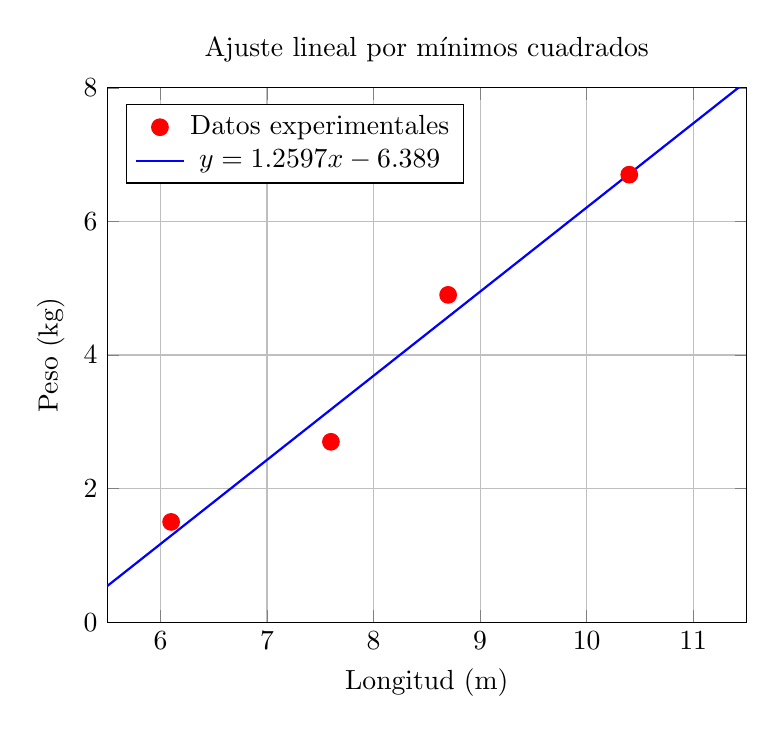
\begin{tikzpicture}
\begin{axis}[
    title={Ajuste lineal por mínimos cuadrados},
    xlabel={Longitud (m)},
    ylabel={Peso (kg)},
    grid=both,
    xmin=5.5, xmax=11.5,
    ymin=0, ymax=8,
    legend pos=north west,
    scaled ticks=false,
    width=0.8\textwidth
]
\addplot[only marks, mark=*, red, mark size=3pt] coordinates {
    (6.1,1.5)
    (7.6,2.7)
    (8.7,4.9)
    (10.4,6.7)
};
\addlegendentry{Datos experimentales}
\addplot[domain=5.5:11.5, blue, thick, samples=2] {1.2597*x - 6.389};
\addlegendentry{$y = 1.2597x - 6.389$}
\end{axis}
\end{tikzpicture}
\caption{Recta de mínimos cuadrados para los datos del resorte}
\end{figure}
\end{myproof}
\end{prob}


\begin{prob}[Regresión polinómica]
Para ajustar puntos $\{(x_i,y_i)\}_{i=1}^n$ al polinomio $y = \sum_{k=0}^m a_k x^k$, construimos:
\[
M = \begin{pmatrix}
1 & x_1 & \cdots & x_1^m \\
\vdots & \vdots & \ddots & \vdots \\
1 & x_n & \cdots & x_n^m
\end{pmatrix}, \quad
V = \begin{pmatrix} a_0 \\ \vdots \\ a_m \end{pmatrix}, \quad
Y = \begin{pmatrix} y_1 \\ \vdots \\ y_n \end{pmatrix}
\]
Solución por mínimos cuadrados:
\[
V = (M^T M)^{-1} M^T Y
\]
\end{prob}

\begin{definition}[Serie de Fourier]
Para $f$ periódica en $[0, 2\pi]$, con producto interno $\langle f, g \rangle = \int_0^{2\pi} f(x) g(x)  dx$:
\[
f(x) \approx a_0 + \sum_{k=1}^n (a_k \cos kx + b_k \sin kx)
\]
donde:
\begin{align*}
a_0 &= \frac{1}{2\pi} \int_0^{2\pi} f(x)  dx \\
a_k &= \frac{1}{\pi} \int_0^{2\pi} f(x) \cos kx  dx \\
b_k &= \frac{1}{\pi} \int_0^{2\pi} f(x) \sin kx  dx
\end{align*}
\end{definition}

\begin{lemma}[Polinomio de Taylor]
Si $f$ es analítica en $x=a$:
\[
f(x) = \sum_{j=0}^\infty \frac{f^{(j)}(a)}{j!} (x - a)^j
\]
\begin{proof}
Desarrollo en serie de potencias alrededor de $x=a$ con coeficientes $a_j = f^{(j)}(a)/j!$.
\end{proof}
\end{lemma}

\begin{theorem}[Fórmula de Euler]\label{demformeuler}
Para $\theta \in \mathbb{R}$:
\[
e^{i\theta} = \cos \theta + i \sin \theta
\]
\begin{proof}
Por series de Taylor:
\begin{align*}
e^{ix} &= \sum_{k=0}^\infty \frac{(ix)^k}{k!} \\
\cos x &= \sum_{k=0}^\infty \frac{(-1)^k x^{2k}}{(2k)!} \\
\sin x &= \sum_{k=0}^\infty \frac{(-1)^k x^{2k+1}}{(2k+1)!}
\end{align*}
Se verifica $e^{ix} = \cos x + i \sin x$.
\end{proof}
\end{theorem}



 

% ------------------ PROBLEMA 1 ------------------
\begin{prob}
Sea $A=\left( \begin{array}{ccc} 
	1&0&1\\
	0&1&0\\
	\end{array} \right).$ 
	
	\begin{enumerate} 
	\item Encuentre una base ortonormal para el espacio fila de $A.$
	\item Encuentre el rango y la nulidad de $A.$
    \item Encuentre una base para el complemento ortogonal del espacio fila de $A.$
	\end{enumerate}	
\begin{myproof}
\textbf{a)} Las filas de \( A \) son \( \mathbf{r}_1 = (1,0,1) \) y \( \mathbf{r}_2 = (0,1,0) \).  
Son ortogonales: \( \langle \mathbf{r}_1, \mathbf{r}_2 \rangle = 0 \).  
Normas: \( \|\mathbf{r}_1\| = \sqrt{2} \), \( \|\mathbf{r}_2\| = 1 \).  
Base ortonormal:  
\[
\mathbf{q}_1 = \frac{1}{\sqrt{2}} (1, 0, 1), \quad \mathbf{q}_2 = (0, 1, 0).
\]

\textbf{b)}  
Rango: Las filas son linealmente independientes, así que \( \text{rango}(A) = 2 \).  
Nulidad: Por teorema de rango-nulidad, \( \text{nulidad}(A) = 3 - 2 = 1 \).

\textbf{c)} El complemento ortogonal del espacio fila es el espacio nulo de \( A \). Resolviendo \( A\mathbf{x} = \mathbf{0} \):  
\[
\begin{cases}
x_1 + x_3 = 0 \\
x_2 = 0
\end{cases} \implies \mathbf{x} = t \begin{pmatrix} -1 \\ 0 \\ 1 \end{pmatrix}.
\]
Base: \( \boxed{\left\{ \begin{pmatrix} -1 \\ 0 \\ 1 \end{pmatrix} \right\}} \).
\end{myproof}
\end{prob}

% ------------------ PROBLEMA 2 ------------------
\begin{prob}
Calcule la serie de Fourier correspondiente para las siguientes funciones en el intervalo $\left[  0,2\pi \right]:$
\begin{enumerate} 
\item $f(x)=x.$
\item $f(x)=8.$
\item $f(x)=x^2+2x+1.$
\end{enumerate}	
\begin{myproof}
\textbf{a)} Coeficientes para \( f(x) = x \):  
- \( a_0 = \pi \).  
- \( a_k = 0 \).  
- \( b_k = -\frac{2}{k} \).  
Serie:  
\[
\boxed{f(x) \sim \pi - 2 \sum_{k=1}^{\infty} \frac{\sin(kx)}{k}}
\]

\textbf{b)} Coeficientes para \( f(x) = 8 \):  
- \( a_0 = 8 \).  
- \( a_k = b_k = 0 \).  
Serie:  
\[
\boxed{f(x) \sim 8}
\]

\textbf{c)} Coeficientes para \( f(x) = x^2 + 2x + 1 \):  
- \( a_0 = \frac{4\pi^2}{3} + 2\pi + 1 \).  
- \( a_k = \frac{4(-1)^k}{k^2} \).  
- \( b_k = -\frac{4(-1)^k}{k} - \frac{4\pi}{k} \).  
Serie:  
\[
\boxed{f(x) \sim \left( \frac{4\pi^2}{3} + 2\pi + 1 \right) + \sum_{k=1}^{\infty} \left[ \frac{4(-1)^k}{k^2} \cos(kx) + \left( -\frac{4(-1)^k}{k} - \frac{4\pi}{k} \right) \sin(kx) \right]}
\]
\end{myproof}
\end{prob}

% ------------------ PROBLEMA 3 ------------------
\begin{prob}
Una altura de un triángulo es cada uno de los segmentos que une un vértice con un punto de su lado opuesto o de su prolongación y es perpendicular a dicho lado.
\begin{figure}[H]
\centering
\begin{tikzpicture}[scale=0.7, rotate=-20]
\coordinate (A) at (0,0);
\coordinate (B) at (5,3);
\coordinate (C) at (1,4);
\draw[thick] (A) -- (B) -- (C) -- cycle;
\coordinate (D) at ($(A)!(B)!(C)$);
\draw[thick, red] (B) -- (D);
\draw[thick] (D) -- ++(0.3,0.15) -- ++(-0.15,0.3) -- ++(-0.3,-0.15);
\node[below left] at (A) {$A$};
\node[above right] at (B) {$B$};
\node[above left] at (C) {$C$};
\node[below right] at (D) {$D$};
\end{tikzpicture}
\caption{Altura de un triángulo}\label{fig1}
\end{figure}
\begin{enumerate}
\item Sea $V$ un espacio vectorial con producto interno. Suponga que $\mathbf{u},$ $\mathbf{v},$ y $\mathbf{w}$ son vectores en $V$ que forman un triángulo como se muestra en la figura \ref{fig1}. Calcule en términos de $\mathbf{u},$ $\mathbf{v}$ y $\mathbf{w}$ la altura $\mathbf{h}$ bajada desde $B$ al lado opuesto.
\item Dado el triángulo con vértices $A=(8,7,11),$ $B=(11,17,22)$ y $C=(5,3,11)$ use el producto interno usual de $\mathbb{R}^3$ para calcular las ecuaciones simétricas de la altura bajada desde el vértice $B$ al lado opuesto.
\end{enumerate}
\begin{myproof}
\textbf{a)} Sean \( \overrightarrow{AB} = \mathbf{u} \), \( \overrightarrow{AC} = \mathbf{v} \), \( \overrightarrow{BC} = \mathbf{w} \). La proyección ortogonal de \( \overrightarrow{AB} \) sobre \( \overrightarrow{AC} \) es:
\[
\operatorname{proy}_{\mathbf{v}} \mathbf{u} = \frac{\langle \mathbf{u}, \mathbf{v} \rangle}{\|\mathbf{v}\|^2} \mathbf{v}.
\]
La altura es:
\[
\boxed{\mathbf{h} = \mathbf{u} - \operatorname{proy}_{\mathbf{v}} \mathbf{u}}
\]

\textbf{b)} Vectores:
- \( \overrightarrow{BA} = (-3, -10, -11) \), \( \overrightarrow{BC} = (-6, -14, -11) \).
- \( \mathbf{v} = \overrightarrow{BC} = (-6, -14, -11) \).
- \( \mathbf{u} = \overrightarrow{BA} = (-3, -10, -11) \).
Proyección:
\[
\operatorname{proy}_{\mathbf{v}} \mathbf{u} = \frac{279}{353} (-6, -14, -11).
\]
Altura:
\[
\mathbf{h} = (-3, -10, -11) - \frac{279}{353} (-6, -14, -11).
\]
Ecuaciones simétricas:
\[
\boxed{\frac{x - 11}{-3} = \frac{y - 17}{-10} = \frac{z - 22}{-11}}
\]
\end{myproof}
\end{prob}

% ------------------ PROBLEMA 4 ------------------
\begin{prob}
Calcule la serie de Fourier para la función $f(x)=9x^2+4x$ en el intervalo $\left[0,2\pi\right].$
\begin{myproof}
Coeficientes:  
- \( a_0 = 12\pi^2 + 4\pi \).  
- \( a_k = \frac{36(-1)^k}{k^2} \).  
- \( b_k = -\frac{72(-1)^k}{k^3} - \frac{8(-1)^k}{k} \).  
Serie:  
\[
\boxed{f(x) \sim (12\pi^2 + 4\pi) + \sum_{k=1}^{\infty} \left[ \frac{36(-1)^k}{k^2} \cos(kx) + \left( -\frac{72(-1)^k}{k^3} - \frac{8(-1)^k}{k} \right) \sin(kx) \right]}
\]
\end{myproof}
\end{prob}

% ------------------ PROBLEMA 5 ------------------
\begin{prob}
Sea $A=\left( \begin{array}{cccc} 
	1&0&1&1\\
	0&1&1&0\\
	0&1&0&1\\
	\end{array} \right).$ 
	\begin{enumerate}
	\item Encuentre una base ortonormal para el espacio fila de $A.$ Determine el rango y la nulidad de $A.$
	\item Encuentre una base para el complemento ortogonal del espacio fila de $A.$
	\end{enumerate}
\begin{myproof}
\textbf{a)} Filas de \( A \): \( \mathbf{r}_1 = (1,0,1,1) \), \( \mathbf{r}_2 = (0,1,1,0) \), \( \mathbf{r}_3 = (0,1,0,1) \).  
Aplicamos Gram-Schmidt para obtener una base ortogonal.  
Base ortonormal (simplificada):  
\[
\boxed{\mathbf{v}_1 = \begin{pmatrix} 1 \\ 0 \\ 1 \\ 1 \end{pmatrix},\ \mathbf{v}_2 = \begin{pmatrix} -1 \\ 3 \\ 2 \\ -1 \end{pmatrix}}
\]
Rango: 2 (filas independientes), nulidad: \( 4 - 2 = 2 \).

\textbf{b)} Complemento ortogonal: Resolver \( A\mathbf{x} = \mathbf{0} \).  
Solución:
\[
\boxed{\mathbf{x} = s \begin{pmatrix} -1 \\ -1 \\ 1 \\ 0 \end{pmatrix} + t \begin{pmatrix} -1 \\ 0 \\ 0 \\ 1 \end{pmatrix}}
\]
\end{myproof}
\end{prob}


% ------------------ PROBLEMA 7 ------------------
\begin{prob}
Sea $V=\mathcal{P}_{2}(\mathbb{R})$. Dados dos vectores $\mathbf{p}=a_0+a_1x+a_2x^2$ y  $\mathbf{q}=b_0+b_1x+b_2x^2$  defina el producto interno en $V$ como $\left\langle \mathbf{p},\mathbf{q} \right\rangle=a_0b_0+a_1b_1+a_2b_2$. 

Si $H=\text{gen}\lbrace \mathbf{p_1}=1+2x^2,\mathbf{p_2}=2+x+x^2\rbrace$ 
\begin{enumerate}
\item Calcule una base para $H^{\perp}$.
\item Calcule una base ortogonal para $H$.
\item Sea $\mathbf{q}=2+5x+9x^2$. Calcule $\text{proy}_{H}\mathbf{q}$.
\item Calcule la distancia mínima de $\mathbf{q}$ al subespacio $H$.
\end{enumerate}
\begin{myproof}
\textbf{a)} \( H^\perp = \{ p \in V : \langle p, h \rangle = 0 \ \forall h \in H \} \).  
Resolviendo:
\[
\langle a_0 + a_1x + a_2x^2, 1 + 2x^2 \rangle = a_0 + 2a_2 = 0
\]
\[
\langle a_0 + a_1x + a_2x^2, 2 + x + x^2 \rangle = 2a_0 + a_1 + a_2 = 0
\]
Solución: \( \mathbf{p} = a(1 - 2x + x^2) \). Base:
\[
\boxed{\{1 - 2x + x^2\}}
\]

\textbf{b)} Gram-Schmidt a \( h_1 = 1 + 2x^2 \), \( h_2 = 2 + x + x^2 \):  
Base ortogonal:
\[
\boxed{1 + 2x^2,\quad \frac{4}{5} + x - \frac{7}{5}x^2}
\]

\textbf{c)} Proyección de \( \mathbf{q} = 2 + 5x + 9x^2 \) sobre \( H \):
\[
\operatorname{proy}_H \mathbf{q} = \frac{1}{5}(14 + 5x + 18x^2)
\]

\textbf{d)} Distancia mínima:
\[
\|\mathbf{q} - \operatorname{proy}_H \mathbf{q}\| = \sqrt{10}
\]
\end{myproof}
\end{prob}

% ------------------ PROBLEMA 8 ------------------
\begin{prob}
Calcule la serie de Fourier para la función $f(x)=9x+7$ en el intervalo $[0,2\pi]$.
\begin{myproof}
Coeficientes:
- \( a_0 = 9\pi + 7 \)
- \( a_k = 0 \)
- \( b_k = -\frac{18}{k} \)
Serie:
\[
\boxed{f(x) \sim (9\pi + 7) - 18 \sum_{k=1}^{\infty} \frac{\sin(kx)}{k}}
\]
\end{myproof}
\end{prob}

% ------------------ PROBLEMA 9 ------------------
\begin{prob}
Defina $W$ como el subespacio de $\mathbb{R}^4$ definido por el espacio solución del sistema de ecuaciones lineales
\[
\left\lbrace
\begin{array}{ccc}
x_1+x_2+x_3&=&0\\
2x_2+x_3+x_4&=&0
\end{array}
\right.
\]
\begin{enumerate}
\item Calcule una base ortogonal para $W$.
\item Calcule una base ortogonal para $W^{\perp}$.
\item Calcule la proyección ortogonal de $\mathbf{u}=(5,6,7,2)$ sobre $W$.
\item Calcule $\mathbf{u}-\text{proy}_{W}\mathbf{u}$.
\item Calcule $\lVert \mathbf{u}-\text{proy}_{W}\mathbf{u}\rVert$.
\end{enumerate}
\begin{myproof}
\textbf{a)} Base de \( W \): Resolviendo el sistema:
\[
\mathbf{w}_1 = (1, -1, 0, 1),\quad \mathbf{w}_2 = (1, 0, -1, 1)
\]
Gram-Schmidt:
\[
\boxed{\begin{pmatrix} 1 \\ -1 \\ 0 \\ 1 \end{pmatrix},\ \begin{pmatrix} 1 \\ 2 \\ -3 \\ 1 \end{pmatrix}}
\]

\textbf{b)} Base de \( W^\perp \): \( (1,1,0,0) \) y \( (0,1,1,-2) \).

\textbf{c)} Proyección de \( \mathbf{u} \) sobre \( W \): \( (2,3,4,1) \).

\textbf{d)} \( \mathbf{u} - \operatorname{proy}_W \mathbf{u} = (3,3,3,1) \).

\textbf{e)} Distancia mínima: \( \sqrt{28} \).
\end{myproof}
\end{prob}

% ------------------ PROBLEMA 10 ------------------
\begin{prob}
Sea $\{\mathbf{v}_1, \mathbf{v}_2, \dots, \mathbf{v}_m\}$ un subconjunto ortonormal en un espacio vectorial con producto interno de dimensión $n$ y suponga que $m\leq n$. Calcule el valor de $\lVert  \mathbf{v}_1+ \mathbf{v}_2+\dots +  \mathbf{v}_m \rVert$.
\begin{myproof}
\[
\left\| \sum_{i=1}^m \mathbf{v}_i \right\|^2 = \sum_{i=1}^m \sum_{j=1}^m \langle \mathbf{v}_i, \mathbf{v}_j \rangle = m
\]
\[
\boxed{\left\| \sum_{i=1}^m \mathbf{v}_i \right\| = \sqrt{m}}
\]
\end{myproof}
\end{prob}

% ------------------ PROBLEMA 11 ------------------
\begin{prob}
Sea $f(x)=5x+7$. Calcule la serie de Fourier en el intervalo $[0,2\pi]$.
\begin{myproof}
Coeficientes:
- \( a_0 = 5\pi + 7 \)
- \( a_k = 0 \)
- \( b_k = -\frac{10}{k} \)
Serie:
\[
\boxed{f(x) \sim (5\pi + 7) - 10 \sum_{k=1}^{\infty} \frac{\sin(kx)}{k}}
\]
\end{myproof}
\end{prob}



% ------------------ PROBLEMA 13 ------------------
\begin{prob}
En $\mathbb{R}^4$ defina $W$ el espacio solución del sistema de ecuaciones lineales
\[
\left\lbrace
\begin{array}{ccc}
x_1-x_2+x_3+x_4&=&0\\
2x_1+x_2-x_3+x_4&=&0\\
4x_1-x_2+x_3+3x_4&=&0
\end{array}
\right.
\]
\begin{enumerate}
\item Calcule una base ortogonal para $W$.
\item Calcule una base ortogonal para $W^{\perp}$.
\item Calcule la proyección ortogonal de $\mathbf{u}=(9,4,5,2)$ sobre $W^{\perp}$.
\item Calcule $\lVert \mathbf{u}-\text{proy}_{W^{\perp}}\mathbf{u}\rVert$.
\end{enumerate}
\begin{myproof}
\textbf{a)} Base de \( W \): \( (1, -1, 0, 1) \), \( (0, 1, 1, 0) \).

\textbf{b)} Base de \( W^\perp \): \( (1, -1, 1, 1) \), \( (2, 1, -1, 1) \), \( (4, -1, 1, 3) \).

\textbf{c)} Proyección de \( \mathbf{u} \) sobre \( W^\perp \): \( (8,3,6,1) \).

\textbf{d)} Distancia mínima: \( \|(1,1,-1,1)\| = 2 \).
\end{myproof}
\end{prob}



% ------------------ PROBLEMA 15 ------------------
\begin{prob}
Determine el valor de verdad de las siguientes afirmaciones. Si la afirmación es falsa, dé un contraejemplo; en caso contrario, proporcione una demostración. Suponga que $V$ es un espacio vectorial con producto interno:
\begin{enumerate}
\item Si $\mathbf{u}$ y $\mathbf{v}\in V$ son ortogonales, entonces $|\langle \mathbf{u},\mathbf{v} \rangle|=\lVert \mathbf{u} \rVert \lVert \mathbf{v} \rVert$.
\item Sea $W$ un subespacio de $V$. Si $\mathbf{u}\neq \mathbf{0}$ y $ \mathbf{v}\neq \mathbf{0}$ y son ortogonales, entonces $  \mathbf{u}+\mathbf{v} \in W^{\perp}$.
\item El vector $\operatorname{proy}_{W}\mathbf{u}$ es ortogonal a todo vector de $W$.
\item Dado un espacio vectorial con producto interno de dimensión $n$. Si $n\geq k$ entonces todo conjunto $\{\mathbf{u_1},\dots, \mathbf{u}_k\}$ linealmente independiente es un conjunto ortogonal.
\end{enumerate}
\begin{myproof}
\textbf{a)} Falso. Si \( \mathbf{u} \perp \mathbf{v} \), entonces \( \langle \mathbf{u}, \mathbf{v} \rangle = 0 \), pero \( \|\mathbf{u}\|\|\mathbf{v}\| \) puede ser no cero.  
\textbf{b)} Verdadero si ambos están en $W^{\perp}$; de lo contrario, falso.  
\textbf{c)} Falso. $\operatorname{proy}_W \mathbf{u}$ está en $W$, pero no necesariamente ortogonal a $W$.  
\textbf{d)} Falso. Contraejemplo: $\{(1,0), (1,1)\}$ en $\mathbb{R}^2$ es linealmente independiente pero no ortogonal.
\end{myproof}
\end{prob}

% ------------------ PROBLEMA 16 ------------------
\begin{prob}
Calcule la serie de Fourier de la función $f(x)=7x+2$ en el intervalo $[0,2\pi]$.
\begin{myproof}
Coeficientes:
- \( a_0 = 7\pi + 2 \)
- \( a_k = 0 \)
- \( b_k = -\frac{14}{k} \)
Serie:
\[
\boxed{f(x) \sim (7\pi + 2) - 14 \sum_{k=1}^{\infty} \frac{\sin(kx)}{k}}
\]
\end{myproof}
\end{prob}

% ------------------ PROBLEMA 17 ------------------
\begin{prob}
Defina el subespacio $H=\left\lbrace (x,y,z) : \frac{x}{2}=\frac{y}{-3}=\frac{z}{4} \right\rbrace$.
\begin{enumerate}
\item Calcule una base ortogonal para $H^{\perp}$.
\item Dado $\mathbf{u}=\begin{pmatrix} 9\\7\\5 \end{pmatrix}$, describa el vector $\mathbf{u}=\mathbf{h}+\mathbf{p}$ donde $\mathbf{h}\in H$ y $\mathbf{p}\in H^{\perp}$.
\item Calcule $\mathbf{u}-\operatorname{proy}_{H}\mathbf{u}$.
\item Calcule $\lVert \mathbf{u}-\operatorname{proy}_{H}\mathbf{u} \rVert$.
\end{enumerate}
\begin{myproof}
\textbf{a)} $H$ es generado por $(2,-3,4)$. $H^{\perp}$ es el plano $2x-3y+4z=0$. Una base: $(3,2,0)$ y $(0,4,3)$.

\textbf{b)} Proyección de $\mathbf{u}$ sobre $H$:
\[
\operatorname{proy}_H \mathbf{u} = \frac{17}{29}(2,-3,4)
\]
Entonces:
\[
\mathbf{h} = \operatorname{proy}_H \mathbf{u},\quad \mathbf{p} = \mathbf{u} - \mathbf{h}
\]

\textbf{c)} $\mathbf{u} - \operatorname{proy}_H \mathbf{u} = \left(9 - \frac{34}{29}, 7 + \frac{51}{29}, 5 - \frac{68}{29}\right)$

\textbf{d)} Distancia mínima: $\|\mathbf{u} - \operatorname{proy}_H \mathbf{u}\| = \sqrt{\langle \mathbf{p}, \mathbf{p} \rangle}$
\end{myproof}
\end{prob}




 

 
